\let\negmedspace\undefined
\let\negthickspace\undefined
\documentclass[journal]{IEEEtran}
\usepackage[a5paper, margin=10mm, onecolumn]{geometry}
\usepackage{lmodern} % Ensure lmodern is loaded for pdflatex
\usepackage{tfrupee} % Include tfrupee package

\setlength{\headheight}{1cm} % Set the height of the header box
\setlength{\headsep}{0mm}     % Set the distance between the header box and the top of the text

\usepackage{gvv-book}
\usepackage{gvv}
\usepackage{cite}
\usepackage{amsmath,amssymb,amsfonts,amsthm}
\usepackage{algorithmic}
\usepackage{graphicx}
\usepackage{textcomp}
\usepackage{xcolor}
\usepackage{txfonts}
\usepackage{listings}
\usepackage{enumitem}
\usepackage{mathtools}
\usepackage{gensymb}
\usepackage{comment}
\usepackage[breaklinks=true]{hyperref}
\usepackage{tkz-euclide} 
\usepackage{listings}
\usepackage{gvv}                                        
\def\inputGnumericTable{}                                 
\usepackage[latin1]{inputenc}                                
\usepackage{color}                                            
\usepackage{array}                                            
\usepackage{longtable}                                       
\usepackage{calc}                                             
\usepackage{multirow}                                         
\usepackage{hhline}                                           
\usepackage{ifthen}                                           
\usepackage{lscape}
\setlength{\parindent}{0pt}
\begin{document}

\bibliographystyle{IEEEtran}
\vspace{3cm}

\title{7-7.2-19}
\author{AI24BTECH11020 - RISHIKA KOTHA}
% \maketitle
% \newpage
% \bigskip
{\let\newpage\relax\maketitle}

\renewcommand{\thefigure}{\theenumi}
\renewcommand{\thetable}{\theenumi}
\setlength{\intextsep}{10pt} % Space between text and floats


\numberwithin{equation}{enumi}
\numberwithin{figure}{enumi}
\renewcommand{\thetable}{\theenumi}
\parindent 0px
Question:Equation of the circle with centre on the Y axis and passing through the origin and the point (2, 3) is
\\
a)$3x^2+3y^2-13y=0$\\
b)$3x^2+3y^2+13x+3=0$\\
c)$6x^2+6y^2-13x=0$\\
d)$x^2+y^2+13x+3=0$\\
\solution
from the given information,
\begin{align*}
	x_1=\myvec{2\\3}, x_2=\myvec{0\\0},n=\myvec{1\\0},c=0 \tag{0.1}
\end{align*}
\begin{align*}
	\myvec{4 & 6 & 1 \\
	       0 & 0 & 1 \\
	       -1 & 0 & 0}
	       \myvec{u\\f}=\myvec{-13\\0\\0}\tag{0.2}
\end{align*}
The augmented matrix is expressed as
\begin{align*}
	\myvec{4 & 6 & 1 & \vrule & -13\\
         0 &  0 & 1 & \vrule & 0\\
	 -1 &  0 & 0 & \vrule & 0} \tag{0.3}
\end{align*}
performing sequences of row operations to transform into Echelon form
\begin{align*}
	\xleftrightarrow[]{R_3 \rightarrow 4R_3+R_1}
	 \myvec{4 & 6 & 1 & \vrule & -13\\
         0 &  0 & 1 & \vrule & 0\\
         0 &  6 & 1 & \vrule & -13} 
	 \xleftrightarrow[]{R_1\rightarrow R_1-R_3}
	 \myvec{4 & 0 & 0 & \vrule & 0\\
	 0 & 0 & 1 & \vrule & 0\\
	 0 & 6 & 1 &\vrule & -13}\\
	 \xleftrightarrow[]{R_2\rightarrow R_2-R_3}
	 \myvec{4 & 0 & 0 &\vrule & 0\\
	 0 & -6 & 0 & \vrule & 13 \\
	 0 & 6 & 1 & \vrule & -13}
	 \xleftrightarrow[]{R_3\rightarrow R_3+R_2}
	 \myvec{4 & 0 & 0 &\vrule & 0\\
	 0 & -6 & 0 & \vrule & 13 \\
	 0 & 0 & 1 & \vrule & 0}\\
	 \xleftrightarrow[]{R_1\rightarrow R_1/4, R_2 \rightarrow R_2/-6}
	 \myvec{1 & 0 & 0 &\vrule & 0\\
         0 & 1 & 0 & \vrule & -13/6 \\
	 0 & 0 & 1 & \vrule & 0} \tag{0.4}
\end{align*}
\begin{align*}
	 u=\myvec{0 \\ -13/6},f=0 \tag{0.5}
\end{align*}
$\therefore$ the equation of the circle is $3x^2+3y^2-13y=0$.
\begin{table}[h!]    
  \centering
  \begin{tabular}[12pt]{ |c| c| c|}
    \hline
	parameter & Description & value \\ 
    \hline
	 C & Centre & $\myvec{0\\ 13/6}$\\
    \hline 
	 O & point1 & $\myvec{0\\0}$\\
    \hline
	 P & point2 & $\myvec{2\\3}$\\
    \hline   
	 r & radius & 13/6\\
    \hline
    \end{tabular}

	\label{7-7.2-19}
\end{table}
\begin{figure}[h!]
	\centering
	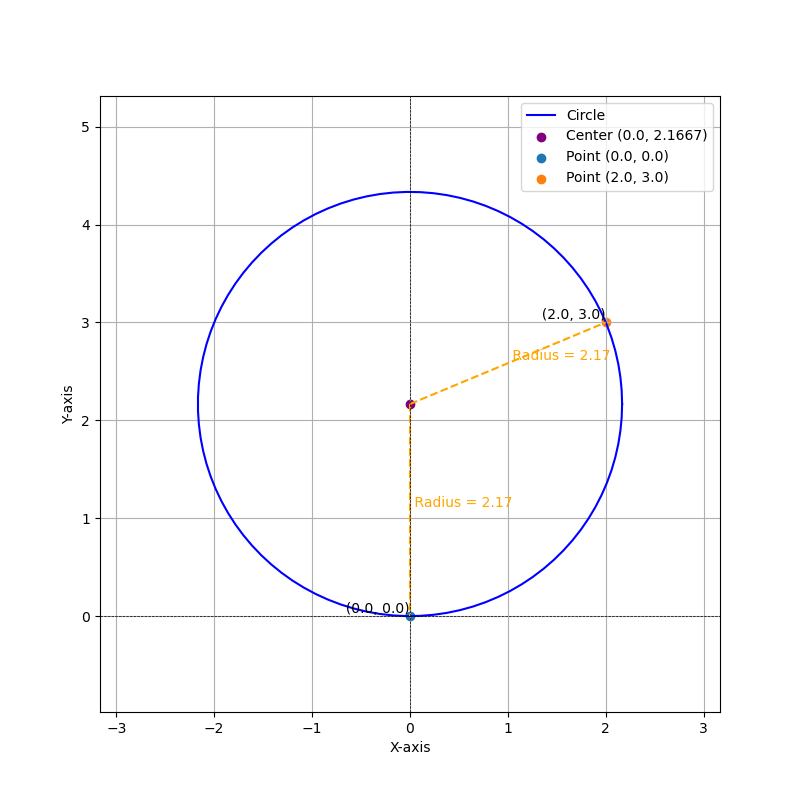
\includegraphics[width=0.7\linewidth]{figs/Fig1.png}
\end{figure}
\end{document}
